% Gerado por scripts/gerar-figuras-monografia.py; não editar.
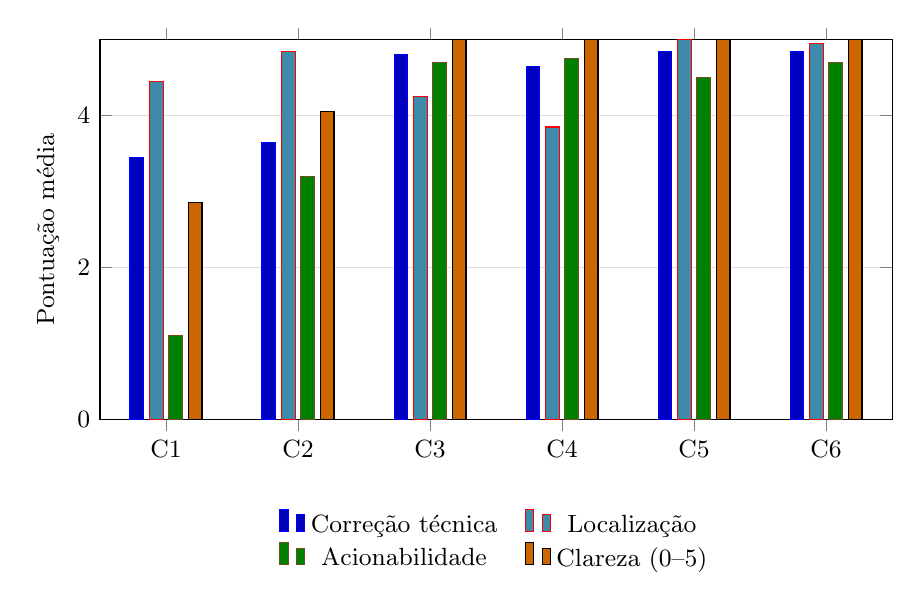
\begin{tikzpicture}
\begin{axis}[
width=0.96\textwidth,height=6.4cm,
tick label style={font=\small},label style={font=\small},
legend style={font=\small,at={(0.5,-0.22)},anchor=north,legend columns=3,draw=none,/tikz/every even column/.append style={column sep=8pt}},
ymajorgrids=true,grid style={black!12},
ybar,bar width=5pt,ymin=0,ymax=5,ylabel={Pontuação média},xtick={1,2,3,4,5,6},xticklabels={C1,C2,C3,C4,C5,C6},enlarge x limits=0.1,legend columns=2
]
\addplot+[ybar,fill=blue!75!black] coordinates {(1,3.45000000) (2,3.65000000) (3,4.80000000) (4,4.65000000) (5,4.85000000) (6,4.85000000)};
\addlegendentry{Correção técnica}
\addplot+[ybar,fill=cyan!65!black] coordinates {(1,4.45000000) (2,4.85000000) (3,4.25000000) (4,3.85000000) (5,5.00000000) (6,4.95000000)};
\addlegendentry{Localização}
\addplot+[ybar,fill=green!50!black] coordinates {(1,1.10000000) (2,3.20000000) (3,4.70000000) (4,4.75000000) (5,4.50000000) (6,4.70000000)};
\addlegendentry{Acionabilidade}
\addplot+[ybar,fill=orange!80!black] coordinates {(1,2.85000000) (2,4.05000000) (3,5.00000000) (4,5.00000000) (5,5.00000000) (6,5.00000000)};
\addlegendentry{Clareza (0--5)}
\end{axis}
\end{tikzpicture}
